\documentclass[border=10pt,tikz]{standalone}
\usepackage{tikz}
\usetikzlibrary{positioning,arrows.meta,shapes}
\begin{document}
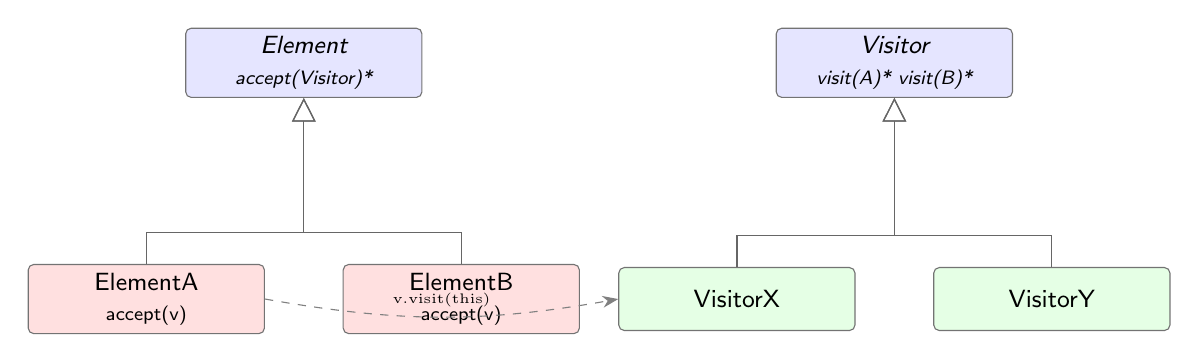
\begin{tikzpicture}[
  font=\sffamily\small,
  cls/.style={rectangle, rounded corners=2pt, draw=black!55, line width=0.4pt,
              minimum height=8mm, minimum width=30mm, inner sep=3pt, fill=white, align=center},
  abs/.style={cls, fill=blue!10, font=\sffamily\itshape\small},
  con/.style={cls, fill=red!12},
  imp/.style={cls, fill=green!10},
  inh/.style={-{Triangle[length=3mm,width=3mm,open]}, draw=black!60, line width=0.45pt},
  arr/.style={-{Stealth[length=2mm]}, draw=black!50, dashed}
]
\node[abs] (e)   at (-3.5, 1.5) {Element \\ \scriptsize accept(Visitor)*};
\node[con] (ea)  at (-5.5,-1.5) {ElementA \\ \scriptsize accept(v)};
\node[con] (eb)  at (-1.5,-1.5) {ElementB \\ \scriptsize accept(v)};

\node[abs] (v)   at ( 4, 1.5) {Visitor \\ \scriptsize visit(A)*  visit(B)*};
\node[imp] (vx)  at ( 2,-1.5) {VisitorX};
\node[imp] (vy)  at ( 6,-1.5) {VisitorY};

\draw[inh] (ea.north) -- ++(0,0.4) -| (e.south);
\draw[inh] (eb.north) -- ++(0,0.4) -| (e.south);
\draw[inh] (vx.north) -- ++(0,0.4) -| (v.south);
\draw[inh] (vy.north) -- ++(0,0.4) -| (v.south);

\draw[arr] (ea.east) to[bend right=10] node[midway, above, font=\tiny]{v.visit(this)} (vx.west);
\end{tikzpicture}
\end{document}
